% THIS IS SIGPROC-SP.TEX - VERSION 3.1
% WORKS WITH V3.2SP OF ACM_PROC_ARTICLE-SP.CLS
% APRIL 2009
%
% It is an example file showing how to use the 'acm_proc_article-sp.cls' V3.2SP
% LaTeX2e document class file for Conference Proceedings submissions.
% ----------------------------------------------------------------------------------------------------------------
% This .tex file (and associated .cls V3.2SP) *DOES NOT* produce:
%       1) The Permission Statement
%       2) The Conference (location) Info information
%       3) The Copyright Line with ACM data
%       4) Page numbering
% ---------------------------------------------------------------------------------------------------------------
% It is an example which *does* use the .bib file (from which the .bbl file
% is produced).
% REMEMBER HOWEVER: After having produced the .bbl file,
% and prior to final submission,
% you need to 'insert'  your .bbl file into your source .tex file so as to provide
% ONE 'self-contained' source file
%
% Questions regarding SIGS should be sent to
% Adrienne Griscti ---> griscti@acm.org
%
% Questions/suggestions regarding the guidelines, .tex and .cls files, etc. to
% Gerald Murray ---> murray@hq.acm.org
%
% For tracking purposes - this is V3.1SP - APRIL 2009

%\documentclass{acm_proc_article-sp}
\documentclass{sig-alternate}
\usepackage[numbers, sort, compress]{natbib}
\usepackage{graphics}
\usepackage{graphicx}
\usepackage{epstopdf}
\usepackage{color}
\usepackage{hyperref}
\usepackage{pdfsync}
\usepackage{mdwlist}

\begin{document}

\conferenceinfo{ECMLS'12,} {}
\CopyrightYear{2012}
\crdata{978-1-4503-0702-4/11/06}
\clubpenalty=10000
\widowpenalty = 10000


%\title{A Sample {\ttlit ACM} SIG Proceedings Paper in LaTeX
%Format\titlenote{(Does NOT produce the permission block, copyright information nor page numbering). For use with ACM\_PROC\_ARTICLE-SP.CLS. Supported by ACM.}}

\newif\ifdraft
\drafttrue                                                                                                   

\ifdraft
% \newcommand{\reviewer}[1]{ {\textcolor{blue}    { ***Reviewer:     #1 }}}
 \newcommand{\jkimnote}[1]{{\textcolor{green}   { ***Joohyun:   #1 }}}
 \newcommand{\jhanote}[1]{  {\textcolor{red}     { ***SJ: #1 }}}
  \newcommand{\pmnote}[1]{  {\textcolor{red}     { ***Pradeep: #1 }}}
 \newcommand{\todo}[1]{  {\textcolor{red}     { ***TODO: #1 }}}
 \newcommand{\fix}[1]{  {\textcolor{red}     { ***FIX: #1 }}}
 \newcommand{\reviewer}[1]{}
\else
 \newcommand{\reviewer}[1]{}
 \newcommand{\jkimnote}[1]{}
 \newcommand{\pmnote}[1]{}
 \newcommand{\jhanote}[1]{}
 \newcommand{\todo}[1]{  {\textcolor{red}     { ***TODO: #1 }}}
 \newcommand{\fix}[1]{}                                                                                     
\fi

\title{Next-Generation Sequencing Reads Alignment Using Pilot-based SAGA-MapReduce}

\numberofauthors{3} %  in this sample file, there are a *total*
% of EIGHT authors. SIX appear on the 'first-page' (for formatting
% reasons) and the remaining two appear in the \additionalauthors section.
%
\author{
% You can go ahead and credit any number of authors here,
% e.g. one 'row of three' or two rows (consisting of one row of three
% and a second row of one, two or three).
%
% The command \alignauthor (no curly braces needed) should
% precede each author name, affiliation/snail-mail address and
% e-mail address. Additionally, tag each line of
% affiliation/address with \affaddr, and tag the
% e-mail address with \email.
%
\alignauthor Pradeep Kumar Mantha\\
       \affaddr{Center for Computation and Technology}\\
       \affaddr{Louisiana State University}\\
       \affaddr{216 Johnston}\\
       \affaddr{Baton Rouge, LA}
       \email{pradeepm66@gmail.com}
\alignauthor Andre Luckow\\
       \affaddr{Center for Computation and Technology}\\
       \affaddr{Louisiana State University}\\
       \affaddr{216 Johnston}\\
       \affaddr{Baton Rouge, LA}
\alignauthor Nayong Kim\\
       \affaddr{Center for Computation and Technology}\\
       \affaddr{Louisiana State University}\\
       \affaddr{216 Johnston}\\
       \affaddr{Baton Rouge, LA}
\and
\alignauthor Joohyun Kim\titlenote{Author for correspondence}\\
       \affaddr{Center for Computation and Technology}\\
       \affaddr{Louisiana State University}\\
       \affaddr{216 Johnston}\\
       \affaddr{Baton Rouge, LA} \\
       \email{jhkim@cct.lsu.edu}
\alignauthor Shantenu Jha\titlenote{Author for correspondence}\\
      \affaddr{Center for Computation and Technology}\\
     \affaddr{Louisiana State University}\\
      \affaddr{214 Johnston}\\
      \affaddr{Baton Rouge, LA}
     \email{sjha@cct.lsu.edu}
}
% There's nothing stopping you putting the seventh, eighth, etc.
% author on the opening page (as the 'third row') but we ask,
% for aesthetic reasons that you place these 'additional authors'
% in the \additional authors block, viz.
%\additionalauthors{Additional authors: John Smith (The Th{\o}rv{\"a}ld Group,
%email: {\texttt{jsmith@affiliation.org}}) and Julius P.~Kumquat
%(The Kumquat Consortium, email: {\texttt{jpkumquat@consortium.net}}).}
\date{25 Feb. 2012}
% Just remember to make sure that the TOTAL number of authors
% is the number that will appear on the first page PLUS the
% number that will appear in the \additionalauthors section.

\maketitle
\begin{abstract} 



 
\end{abstract}

We present the use of MapReduce programming model for Next-Generatiion Sequencing (NGS) data analysis.  Our approach is based on Pilot-based SAGA-MapReduce (P-SAGA-MR) framework which extends previously introduced SAGA-MapReduce with a Pilot task and data management implementation.  With the new P-SAGA-MR, a variety of applications for NGS data and downstream analysis are transformed to become scalable tools by analyzing and processing large distributed data sets located in distributed multiple infrastructures effectively.   As an example, we demonstrate the capacity of P-SAGA-MR for an application carrying out NGS reads alignment and duplicate removal, implemented to the map phase and the reduce phase task, respectively.  We compared our implementation with other MapReduce-based NGS data analysis tools such as SEQAL of the SEAL package and Crossbow that make use of Hadoop-based environment but currently implemented with two different mappers, BWA and Bowtie, respectively.  Based on obtained results presenting benchmark experiments using two different mappers and comparison to the two tools, we discuss how P-SAGA-MR stands out, in particular with respect to the scalability with multiple cluster integration and the extensibility with supporting multiple tools and the potential of P-SAGA-MR for a broad range of NGS data analytics. 


\category{D.1.3}{Software}{Concurrent Programming}{ Distributed
  programming/parallel programming} \category{J.3}{Computer
  Applications}{Bioinformatics, Mapping}


% A category with the (minimum) three required fields
%\category{H.4}{Information Systems Applications}{Miscellaneous} %Acategory including the fourth, optional field follows...
%\category{D.2.8}{Software Engineering}{Metrics}[complexity measures,performance measures]

\terms{Design, Experimentation, Performance}

 \keywords{Genome Sequence Alignment, BWA, Human Genome, RNA-Seq Data,
  MapReduce, Distributed Computing, Simple API for Grid
  Applications (SAGA), Pilot Job and Data}

%\keywords{ACM proceedings, \LaTeX, text tagging} % NOT required for Proceedings 
%\keywords{RNA conformation energy landscape, Runtime Environment, SAM-I riboswitch,
% S gene of Bovine Corona Viral Genome} % NOT required for Proceedings

\section{INTRODUCTION} 
Recent advances in high-throughput DNA sequencing technologies such as Next-Generation Sequencing (NGS) platforms have  imposed unprecedented challenges in areas of bioinformatics, computational biology, and biocomputing in general\cite{metzker2010,1000genome,wang2009-natrevgen,alex2009,mcpherson2009}.  With astronomically explosive volumes of raw data and processed data, along with required computational tasks that often need scalable infrastructure, these challenges are to some extent novel because of the need of an integrative solution leveraging algorithmic advances, computational implementations, and infrastructure developments altogether. Indeed, still at this moment it is common to find many biologists who have sequencing data sets in his/her hand for their biological/biomedical queries but are puzzled surrounded with so-many-tools implemented with specific algorithms and computational requirements including the installation, maintenance, and update of the software tools. 

Among many directions for responding to such challenges, the use of parallelism is an essential strategy and in fact the programming model of MapReduce has been widely touted as an efficient solution for big data problems\cite{mapreduce-2004-dean}.  Several tools using MapReduce were already introduced in NGS data analysis such as read alignment onto a reference genome\cite{cloudburst, gatk,langmead2009,seal2011,langmead2010, taylor2010}.

In this work, we present the development of a Next-Generation Sequencing reads alignment tool using Pilot-based SAGA-MapReduce (P-SAGA-MR or PMR) which is a recent re-implementation of SAGA-MapReduce with a newly developed Pilot-based approach\cite{Sehgal2011590,pmr2012}.  Indeed, P-SAGA-MR provides a viable solution for computational challenges with NGS data analytics, in particular, arising from the required scalability for dealing with ever-growing data volume, variety, and demand for time-to-solution.  Our implementation of the MapReduce programming model supports the development of dynamic applications which represent applications executed in distributed resources via effective and dynamic task and data management, which is contrasted to other approaches using Hadoop-based MapReduce implementations\cite{cloudburst,langmead2009,seal2011,langmead2010}.  With a specific example, in this work we demonstrate how PMR has the capacity for executing a task of NGS data analysis effectively with recognizing aspects associated with algorithms, implementations, and infrastructure.

The target task is the combination of reads alignment and duplicate removal, with which we examine the characteristics and the performance of the developed tool specifically in distributed computing environments.  The discussions including the potential of this approach for a broad range of NGS data analytics are presented.  Also, we compare our implementation with other approaches that implemented conventional MapReduce with Hadoop.

Before we present the contribution and outline of the paper, we
clarify our usage of the different types of scaling that this paper
will be concerned with: {\it scale-up} -- or the most common type of
scaling behavior, is a reference to the ability (performance) of using
many cores efficiently; {\it scale-out} is a measure of the number of
tasks that can be concurrently executed \& managed; {\it scale-across}
is a measure of the number of distinct compute resources that an
application can utilize.

\pmnote{
Doesn't  scale-up and scale-out mean same thing as per above description??
In Fig 3,  as the number of nodes or cores increase, the runtime decreases- so its scales-up well.
The concurrency of tasks, increase with number of cores.. Figure -3 again shows that.
I mean both are related to the number of workers used.
}

\jhanote{Say something about tooling, something about integrated the concurrency also increased. and
  extensible environment}

\jhanote{`Unfortunately, users cannot directly deploy a MapReduce
  framework such as Hadoop on top of these clusters to form a single
  larger MapReduce cluster. Typically the internal nodes of a cluster
  are not directly reachable from outside. However, MapReduce requires
  the master node to directly communicate with any slave node, which
  is also one of the reasons why MapReduce frameworks are usually
  deployed within a single cluster. Therefore, one challenge is to
  make multiple clusters act collaboratively as one so it can more
  efficiently run MapReduce.''}

\pmnote{Why do we need a distributed mapreduce framework to process
  distributed data on multiple frameworks?  1. To process the data on
  a single cluster takes more time and getting shared HPC resources to
  process that huge is also difficult. So distributing the data( Which
  can be a one time setup) to multiple clusters allows the flexibility
  to use more computation and process the data quickly.  2. "Although
  commercial clouds can provide virtually unlimited computation and
  storage resources on-demand, due to financial, security and possibly
  other concerns, many researchers still run experiments on a number
  of small clusters with limited number of nodes that cannot unleash
  the full power of MapReduce." - {Hierarchical mapreduce} }

The paper is organized as follows. In the following section, the data sets we used for this work and the introducing of the P-SAGA-MR are presented.   Later, results for parallel performance measurements and comparison of our results with SEQAL which represents applications that use the open source Hadoop-based MapReduce\cite{hadoop-url, taylor2010} and aiming the same read alignment-duplicate removal task\cite{seal_2011_mapred,seal2011} are presented.  Finally, we will give concluding remarks focusing on challenges associated with scalable calculations of NGS data analytics which could be effectively resolved by the utilization of P-SAGA-MR that seamlessly supports parallel/concurrent computation and data processing  tasks with scalable multiple HPC infrastructures.

\begin{center}
\begin{table*}[ht]
{\small
\hfill{}
\begin{tabular}{|l|l|c|c|c|c|c|c|}
\hline
  & \textbf{P-SAGA-MR}\cite{pmr2012} & \textbf{SEQAL}\cite{seal2011} & \textbf{Crossbow}\cite{langmead2009} & \textbf{CloudBurst}\cite{cloudburst} & \textbf{GATK}\cite{gatk} \\ \hline
%\cline{3-9}
 \hline 
Key Parallelism   & Pilot-based   &  Hadoop-based/  &  Hadoop   & Hadoop-based & MR-based Structured \\ 
Stretegy  & Distributed MR & MR  & Streaming  & MR & Programming  \\
& & (Pydoop) &  & & Framework  \\ \hline
  
Hadoop & No & Yes & Yes\footnote[1] & Yes & No \\ 
Requirement  & & & &  &\\ \hline  
  
    
Multiple  Cluster & Yes  & Limited   & Limited  & Limited  & Limited \\
Support &  & by Hadoop &  by Hadoop & by Hadoop  & by JVM   \\ \hline

Distributed Job and  & Advert Service (SAGA) & Hadoop/HDFS & Hadoop/HDFS & Hadoop/HDFS & Java \\ 
Data Coordination & &  & & & Framework\\ \hline
%Strength & 1. Scalable with Multiple Systems  &  &  &  & \\ 
%
%&  2. Pilot Job/Data Support & &  & & \\ 
%&3. Extensibility  &  &  &  & \\
%& 4. Short Development Cycle & & & & \\\hline
%Weakness &  & 1. HDFS Limitations & 1. HDFS Limitations & 1. HDFS Limitations  &\\ \hline

Primary Aligner &  BWA  &  BWA & Bowtie & RMAP &  BWA \\ \hline
Multiple Aligner  & Straightforward & Not Straight- & Possible & Not Straight-  & Straight-  \\ 
Support &  & forward &   & forward  & forward \\\hline
Primary Tasks & Alignment/Duplicate  & Alignment/ & Alignment/ & Alignment &Various\\
  &  Removal & Duplicate & SNP Discovery & & NGS Data  \\  
           &  &  Removal & &  & \& Downstream  \\
           &  & & &  & Analysis \\ \hline  
Extensibility for   &  High  & Medium &  Low & Low & High      \\
Multiple Tools  &      &  &  &  &   \\ \hline

\hline
\end{tabular}}
\hfill{}
\caption{Feature comparison of P-SAGA-MR with other tools for Next-Generation Sequencing (NGS) data analysis with MapReduce framework.  $^{1}${Crossbow can run without hadoop when scalability is not needed.} }
 \label{table:mr-comparison}
\end{table*}
\end{center}

\section{Materials and Methods}
\subsection{NGS Data Sets and Analysis}
The short reads alignment, along with assembly, is the first step in every pipeline projects aiming biological discovery with sequencing data from NGS platforms.  Since the de-novo assembly remains still challenging at this moment primarily due to the short length of sequencing reads from NGS machines, alignment or mapping is taken as the first task in most of cases.  After alignment, duplicate read removal might be required because the preparation step artifacts stemming from high-throughtput read amplification might introduce many duplicates that are not relevant to true biological conditions.  These two steps could be parallelized by using MapReduce such that the read alignment step is conducted as a Map phase and duplicate removal as a Reduce phase.  Note that a certain kind of variation for designing MapReduce-based analysis for NGS data is also of interest considering the duplicate removal task might be skipped or replaced with other analysis tasks such as SNP finding, transcript quantification or peak calling that are required for other advanced NGS protocols.  The development for such topics will be announced in the future works.

For this work, we used RNA-Seq data from our collaborator lab which is from human lymphoma cell lines.  A brief summary on the data set is given in Table~\ref{table:data}

\subsection{Experimental Set-up for NGS Read Alignment and Duplicate Removal}
\subsubsection{Pilot-based SAGA-MapReduce}
For this work, we used two Futuregrid systems, SIERRA and HOTEL.  More details on the specification of these machines can be found from the web page of Futuregrid\cite{futuregrid_url}.  


\subsubsection{Comparative Experiment with SEQAL}
SEQAL is chosen for the comparison with our approach with P-SAGA-MR since it aims the analysis of read alignment and duplicate removal.  Also, SEQAL is implemented with BWA for alignment, implying that the comparison is informative to differentiate Hadoop-based MR implementation and the Pilot-based implementation.

Hadoop version 0.20.2 and seqal version  seal-0.2.3 were used for SEQAL-based read alignment.

First of all, PJ based mapreduce involves advert coordination- whereas HDFS filesytem involves TCP/IP layer for communication between data nodes; and job nodes use RPC to communicate between each other.
Note that it is not easy for Hadoop/Normal MR to be scaled out to multiple clusters(unless and until clusters have some common global filesystem, which is rare and involves latency issues).  On the contrary, PMR supports  multiple clusters and no need of having common filesystem by design.

Hadoop SEQAL experiment setup is as follows.  The input file format is prq format.  SEAL, a software tool containing SEQAL as a part, has a file conversion capacity between qseq/fastq and prq format.  The replication factor for Hadoop configuration is set  to 1.

To make the comparision more meaningful, we set the number of nodes as 4, and the maximum map and reduce tasks is set to be 2.  We found that if the number of tasks is set to be more than 2, the issue with memory size occurred.  \pmnote{refer to reference paper}  Thus, total 8 workers were used.
The chunk size used is 128MB, which is default block size and corresponding to nearly 292,763 reads.
The reduce phase starts after all map phase tasks are completed. 

PMR setup for using two separated systems is as follows.  Initially the half of the data is placed on sierra. whereas the remaining half is on hotel. The number of workers is 8 and each individual node of the four nodes (two nodes per each cluster) has 2 workers.  For a single system set up, everything is similar except all workers are now running in the system.  Input is in fastq format. An In-house script is used for the chunking step. The user can define the chunker script and provide as an input to the pMR framwork.  
 
   \pmnote{chunksize = number of lines of fastq file ( number of sequences (292763 * 4 ) since in fastq each sequence is of 4 lines..
tts = max( map on sierra, map on hotel)+max( time tansfer from sierra to hotel, time transfer from hotel to sierra)+max(reduce on sierra, reduce on hotel)..
Graph : x axis- (2,4,8 input sizes) with chunk size 292763 sequences, number of workers=8, reduces=8.
experiments repeated thrice.. }
 
For the experiment using distributed resources, all input and required data are stored initially on a single cluster to process.  Again, Hadoop-based implementation, SEQAL cannot run on multiple clusters and thus all experiments are conducted in a single Hadoop-installed system.

We calculated the time-to-solution (tts) as the combination of the time for transferring data to A cluster from B cluster (when A and B are used) and SEQAL execution time. 
 


\section{Experiments}

\jhanote{need to explain which/what expeirments, how we perform them,
  and why?}

\jhanote{Motivation: distributed data requirements; MR-based sequncing
  applications comparision; challenges of the former in the latter}

\section{Results}

\subsection{Pilot Model-driven SAGA-MapReduce for NGS data analysis: Implementation}
In Fig.~\ref{fig:arch-pj-saga-mr}, the overall architecture of PJ-based SAGA-MapReduce for reads alignment and duplicate removal tasks is shown.  In brief, the target tasks are carried out with this order. 1.SAGA-MapReduce launches Map tasks on N clusters using Pilot-Job 2. After the Map stage, SAGA-MapReduce exchanges Intermediate data between clusters using Pilot-Data  3. SAGA-MapReduce launches Reduce tasks on N clusters using Pilot-Job.


\begin{figure}
 \centering
%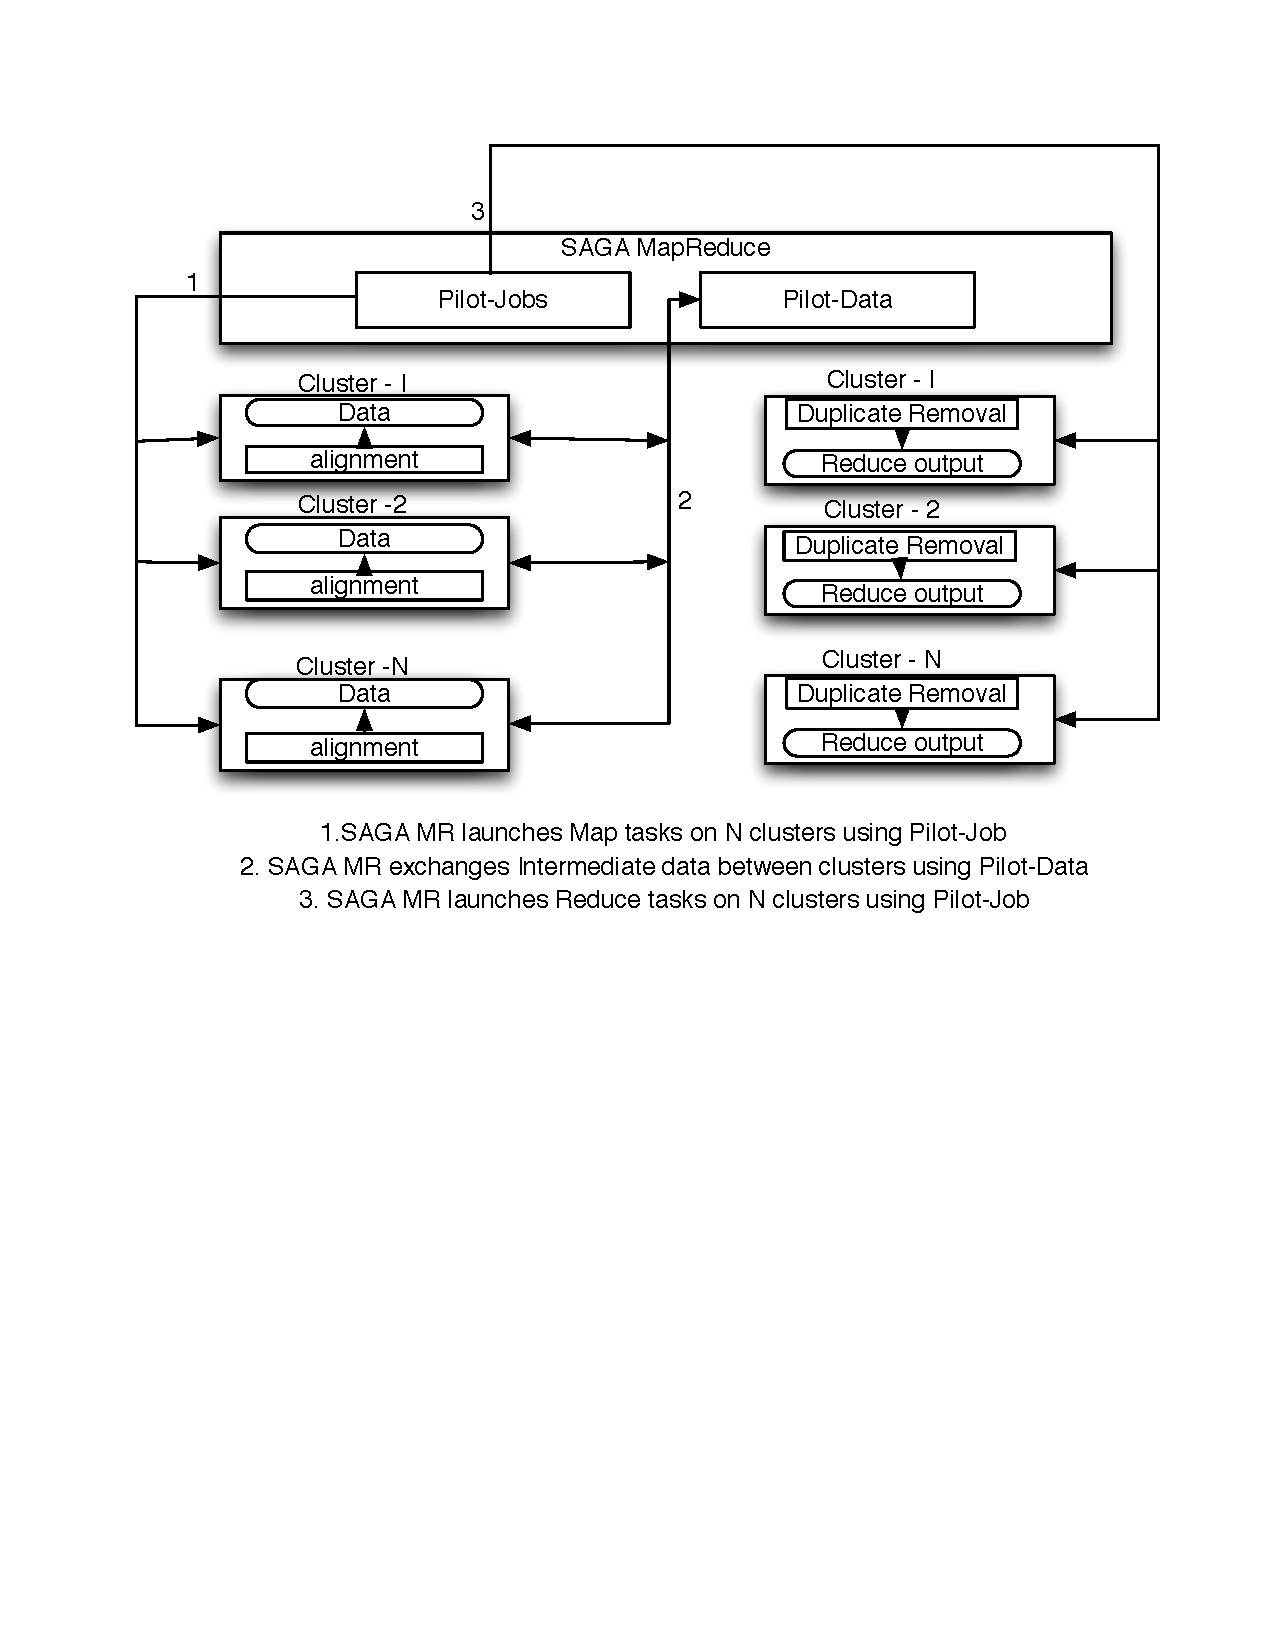
\includegraphics[scale=0.45]{figures/align-dup.pdf} 
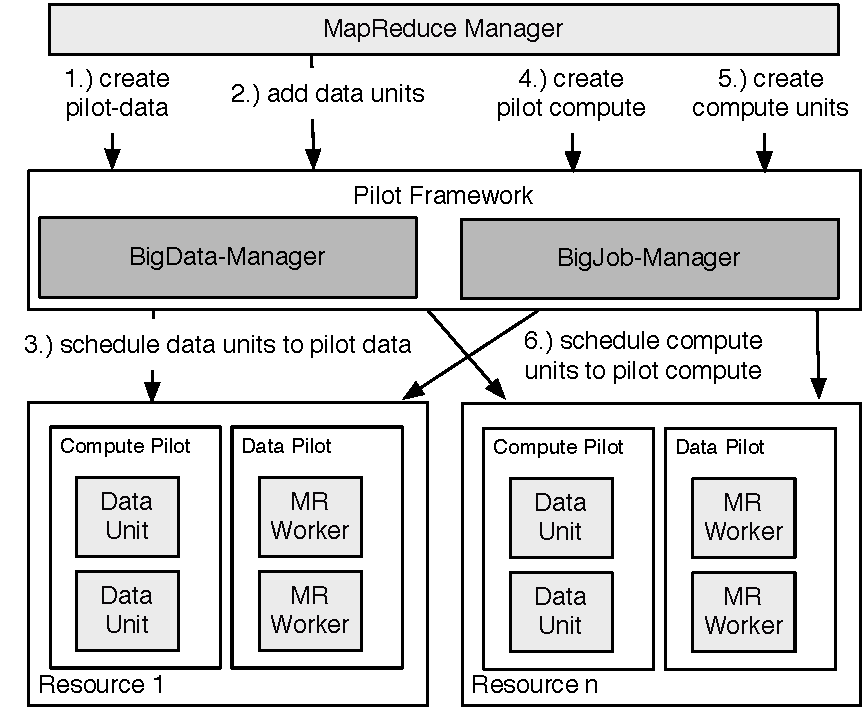
\includegraphics[scale=0.45]{figures/mapreduce-pilotdata.pdf} 
\caption{\small Pilot-SAGA MapReduce architecture}
  \label{fig:arch-pj-saga-mr} 
\end{figure}


\subsection{Pilot Model-driven SAGA-MapReduce for NGS data analysis : Reads Alignment and Duplicate Removal}

There are unique features that differentiate our approach from others, which could be beneficial for developing cyberinfrastructure for NGS data analytics and downstream analysis.  
\begin{enumerate}

\item Pilot-based MapReduce for Parallel/Concurrency framework 
\item No need of Hadoop infrastructure
\item Scalability by utilizing multiple compute resources
\item Distributed data across distributed resources
\end{enumerate}
 
 \begin{figure}
 \centering
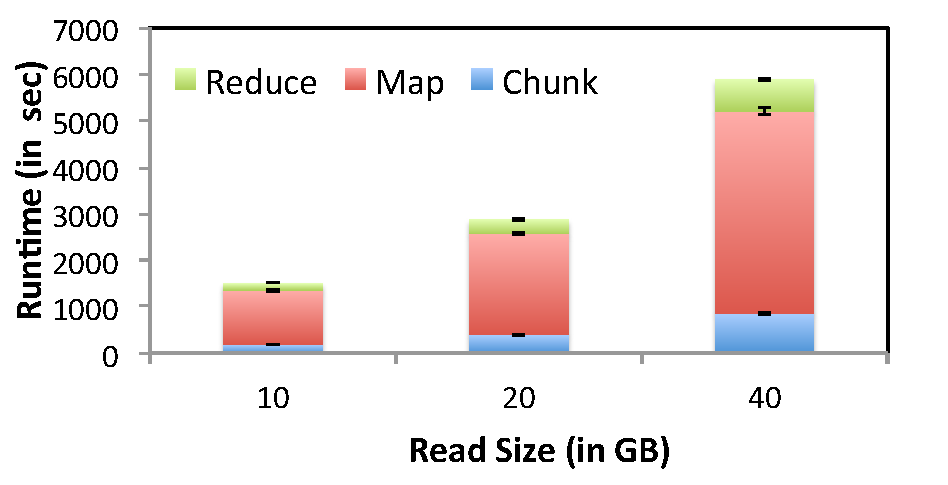
\includegraphics[scale=0.50]{figures/pj-smr-tts.pdf} 
\caption{\small Scale-out: Read size dependent time-to-solution.  The number of nodes for this experiment is 16, and chunk size is set to contain 62500 reads.  The number of reducers is set to 8}
  \label{fig:read-size} 
\end{figure}

 In Fig.~\ref{fig:read-size}, the required scalability is measured with the increase of input data size.  It is apparent that compared to the map phase that conducts parallel alignment with BWA, other two steps, the reduce phase and the preparation of input data with multiple files are negligible.  Note that the alignment and the duplicate removal tasks are low-aggregation problems for MapReduce framework.  

Meanwhile, Fig~\ref{fig:scale-p-saga-mr} shows the overall good scaling results for the task of mapping and duplicate removal with P-SAGA-MR as the number of nodes used increases, indicating that P-SAGA-MR is a viable framework for delivering the good parallel performance against sizable data sets.





\begin{figure}
 \centering
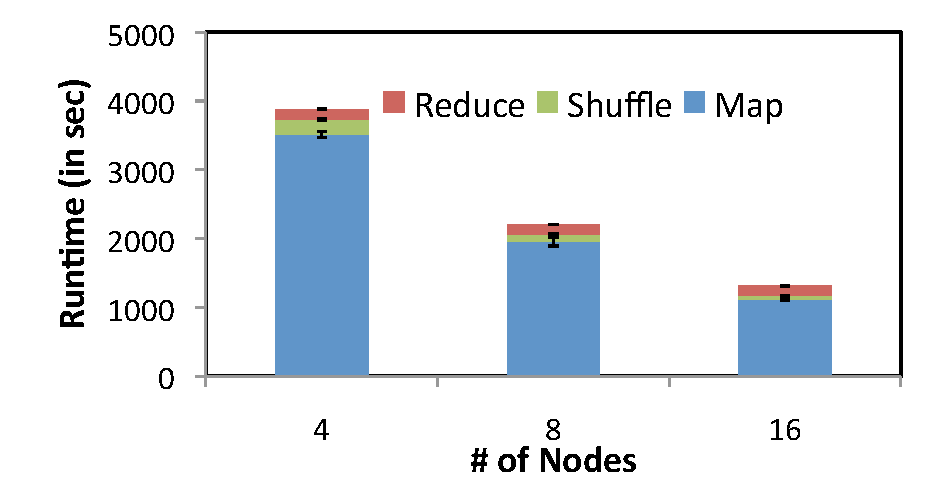
\includegraphics[scale=0.50]{figures/pj-smr-scale.pdf}
\caption{\small Scale-up: Pilot-based SAGA-MapReduce scalability; As the number of nodes increases, number of workers/node=2, the time to solution decreased, the input read size is 10GB, number of reduces is set to 8, number of reads/chunk = 625000. }
  \label{fig:scale-p-saga-mr} 
\end{figure}


\subsection{Comparison to Hadoop-based SEQAL and Crossbow}
\subsubsection{Closely Related Works}
There exist a few works specifically targeting NGS data analytics using the MR framework and four other tools are presented in Table~\ref{table:mr-comparison}.  In brief, Cloudburst was one of early tools to demonstrate the significant potential of MapReduce for NGS data analysis, whereas Crossbow focused on better scalability using Hadoop streaming.  Compared to the two Hadoop-based tools, GATK was introduced to support the general parallel execution pattern across many NGS data analytics.  Recently, the SEAL package was announced in which SEQAL is a utility for the alignment and duplicate removal.   

In spite of the commonality that MapReduce is the core programming model for the tools, they differ in several aspects depending upon the need of Hadoop, the way to utilize Hadoop, the level of flexibility for the extension of tools for alternative tasks or external tools such as aligners, and multiple cluster support.

Interestingly, multi-domain support with the MR framework is recently demonstrated for AutodDock application which is, in contrast to our applications that are loosely-coupled, pleasingly parallel.\cite{ecmls11-mr-autodock}

\begin{figure}
 \centering
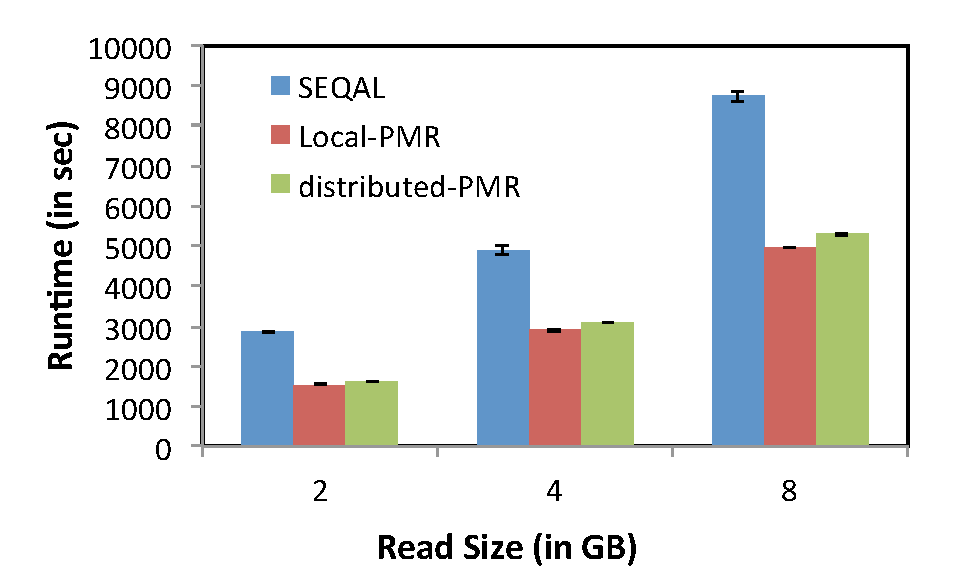
\includegraphics[scale=0.50]{figures/seqalvslocalpmr.pdf}

\caption{\small Hadoop-based SEQAL vs. Local-PMR vs. distributed-PMR.  BWA is the aligner for the map phase; number of nodes=4; number of workers/node=2, number of reducers=8, number of reads/chunk=292763 for PMR ==128MB for hadoop based apps}

  \label{fig:comp_with_seqal_1} 
\end{figure}

\subsubsection{Performance Comparison}
In Fig.~\ref{fig:comp_with_seqal_1} and Fig.~\ref{fig:comp_with_seqal_2}, we compared directly the time-to-solution between SEQAL and two scenarios with P-SAGA-MR, one with a single cluster and the other with two clusters.  In Fig.~\ref{fig:comp_with_seqal_2}, we dissect the contributions of each step for the total runtime.  

Notably, SEQAL takes more time on the overall run time, and the most contributing cause come from the map phase.  We interpret this result with the fact that the tmp directory on each node is used to store data by hadoop, but when the size of a tmp directory is limited for the required task, a remote file system is configured as  the tmp data directory for remote disks of other nodes.

Another observation from Fig.~\ref{fig:comp_with_seqal_1} and Fig.~\ref{fig:comp_with_seqal_2} is that whereas SEQAL is limited by a single cluster with Hadoop, P-SAGA-MR can be easily scale-across multiple clusters. The distributed-PMR is indeed performing well against local-PMR without significant performance loss due to the low connectivity between two clusters with our experimental set up.  

Again, Fig.~\ref{fig:comp_with_seqal_2} clearly indicates the map phase for SEQAL has a disadvantage against P-SAGA-MR.  The comparison of the reduce phase could originate from the different implementation between SEQAL and ours.

\begin{figure} 
 \centering
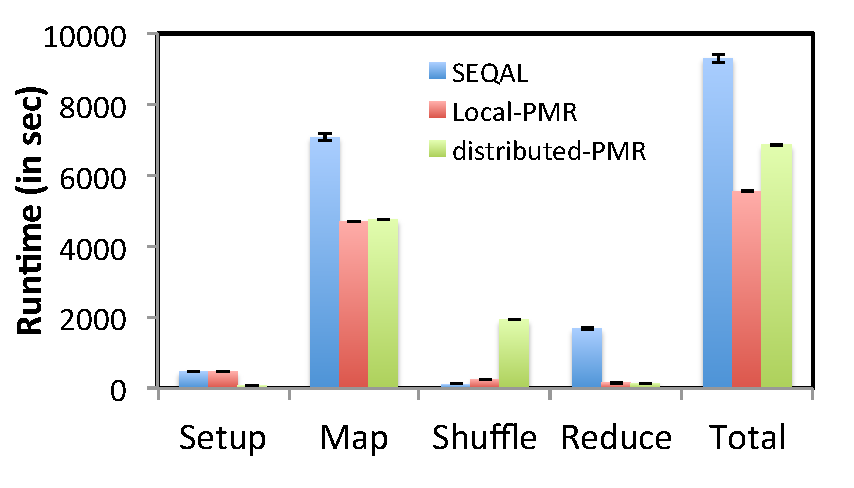
\includegraphics[scale=0.50]{figures/8GB_phasewisetimes.pdf}
\caption{\small  Alignment and Duplicate Read Removal on 8GB input data.  Comparison between SEQAL vs. Local-PMR vs. distributed-PMR.  The runtime contributions from each step are compared in details. BWA is the aligner for the map phase; ********DMR provides scale-across********** as two machines sierra and hotel are used.}
  \label{fig:comp_with_seqal_2} 
\end{figure}


\begin{figure} 
 \centering
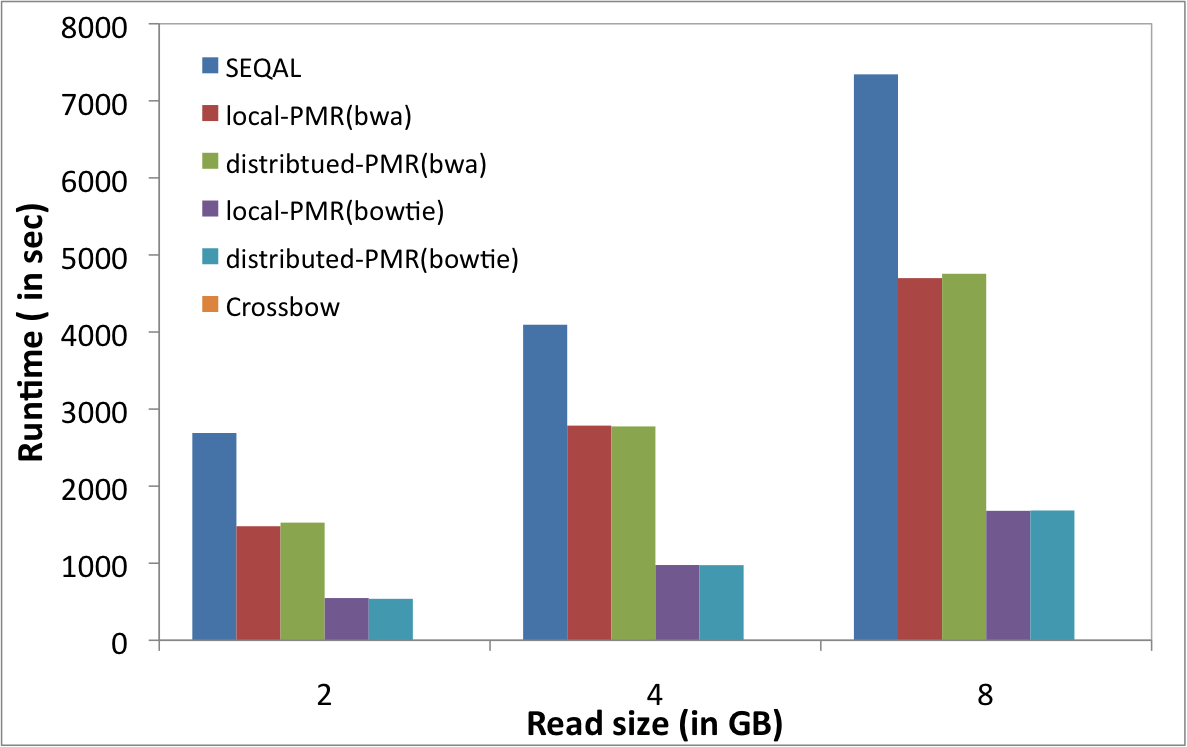
\includegraphics[scale=0.50]{figures/tool_comp.png}
\caption{\small  Map phase comparision of SEQAL, Local-PMR(BWA), distributed-PMR(BWA), Local-PMR(Bowtie), distributed-PMR(Bowtie).  
number of nodes=4, number of workers/node=2,reduces=8, number of reads/chunk=292763; ********DMR provides scale-across********** as two machines sierra and hotel are used.}
  \label{fig:tool_comp} 
\end{figure}



As the number of input sequences increased the time to solution also increased linearly for both SEQAL and local-PMR. 
The time to solution decreased by an average of 43.39\% with 95\% confidence interval of 3.03\%. The Map phase of Local-PMR is on an average of 64\% of Map phase of SEQAL application, and is reduced by an average of 35.7\%
The reduce phase is very less compared to seqal applicaiton because there is not sort involved in reduce phase.
\pmnote{( why is that?? i dont see any reason to have a sort before reduce starts)) we do sort intermediate data before shuffled.}
The reduce phase is average of 8.85\% of reduce phase of seqal  ( it involves sort )

\pmnote{how to explain performance of PMR ??}..One of the performance bottlneck for PMR is coordination system used... we used redis as coordination system... which is proved best ,when compared to other coordination systems{Pstar reference}. I think we can compare the results.. but cant say why SEQAL performed better.. since, it needs understanding of how SEQAL actually works.


\section{Discussions and Concluding Remarks}
\textit{P-SAGA-MR vs. Other approaches}
\\

On the other hand, in spite of many advantages including fault-resilency and easy scalability within a cluster, Hadoop-based approaches such as Crossbow, Cloudburst, and SEAQL are also limited by the nature of Hadoop.  Firstly, the overall performance of Hadoop-based MapReduce is determined by the unknown network performance and the connectivity between the data storage and the compute which are determined by characteristics of the cluster Hadoop is installed.  The tight coupling between the MapReduce applications with underlying Hadoop causes unnecessary complexity when the optimization or the design of parallel execution is required.  Secondly, it is not trivial to scale across different clusters.  Many issues on the connectivity between two separate clusters including firewalls, different security policies, and potentially different administration structure are making difficult to extend Hadoop with other cluster systems.  Thirdly, it is a still ongoing concern that Hadoop's current implementation has obstacles from the scalability issue with the design with Namenode and Job tracker.   The open source Hadoop is implemented with a job and task tracker: the job tracker is the central manager that dispatches map and reduce tasks to the nodes(nodes could be from multiple clusters) of the Hadoop cluster. On each node the task tracker is responsible for executing the respective tasks. The main limitation of this architecture is the fact that it intermixes both cluster resource management and application-level task managements. Thus, it is e.g. not easily possible to integrate Hadoop with another resource management tool, e.g. PBS or Torque. Also, the job tracker represents a single point of failure and scalability bottleneck. Another limitation is the latencies between machines should not be so big as HDFS uses Avro - an RPC-style protocol for communications.

Collectively, P-SAGA-MR has edges in terms of flexibility and non-Hadoop-based architecture

\textit{P-SAGA-MR, a viable solution for scale-across and extensible framework for NGS data analytics}
\\

\textit{DARE and beyond}





\section*{Acknowledgement}
This document was developed with support from the National Science
Foundation (NSF) under Grant No.  0910812 to Indiana University for
``FutureGrid: An Experimental, High-Performance Grid Test-bed.''  We
also acknowledge the SEAL developer, Luca Pireddu for useful performance related
discussions, and Erik Flemington for allowing us to use his RNA-seq data sets. Computing resources were made possible via NSF TRAC award TG-MCB090174 and LONI resources.  The project described was partially
supported by Grant Number P20RR016456 from the NIH National Center For
Research Resources.

\bibliographystyle{abbrv} 
\bibliography{compbio,saga}


\end{document}

Any opinions, ndings, and conclusions or recommendations expressed in
this material are those of the author(s) and do not necessarily
reflect the views.
